\chapter{الكهرسلبية والقطبية والقوى بين الجزيئات}\label{ch:g11:polarity-and-cohesion}

يجري الوزغ صاعدًا على لوح نافذة ويتدلى من الزجاج بإصبع واحدة، بلا غراء ولا
ممصّ. \omterm{def:g7:atoms-and-molecules:molecule}{وجزيء} الماء، \ce{H2O}، أخف من \omterm{def:g7:atoms-and-molecules:molecule}{جزيء} كبريتيد الهيدروجين، \ce{H2S}، ومع ذلك
يغلي الماء عند \qty{100}{\celsius} بينما يبقى كبريتيد الهيدروجين غازًا حتى
\qty{-60}{\celsius}. والقصتان تدوران حول الشيء نفسه: القوى التي تشد \omterm{def:g7:atoms-and-molecules:molecule}{الجزيئات}
بعضها إلى بعض، وإلى أشياء أخرى. وهي أضعف بكثير من الروابط التساهمية داخل
\omterm{def:g7:atoms-and-molecules:molecule}{الجزيء}، لكنها تقرر هل تكون المادة غازًا أم سائلًا أم جسمًا صلبًا في درجة حرارة
الغرفة، وهل يسقط الوزغ.

\begin{recall}
\omterm{def:g10:lewis-and-shape:covalent-bond}{الرابطة التساهمية} زوج من \omterm{def:g9:inside-the-atom:nucleus}{الإلكترونات} تتشارك فيه ذرتان؛ وبنى لويس تُظهر الأزواج
الرابطة والأزواج الحرة، والأزواج حول \omterm{def:g7:atoms-and-molecules:atom}{الذرة} المركزية تقرر شكل \omterm{def:g7:atoms-and-molecules:molecule}{الجزيء}
(\cref{ch:g10:lewis-and-shape}). \omterm{def:g9:ions:ion}{والأيونات} تحمل شحنة؛ وفي الجسم الصلب الأيوني
تتجاذب \omterm{def:g9:ions:ion}{الأيونات} الموجبة والسالبة (\cref{ch:g9:ions}).
\end{recall}

\begin{omfigure}
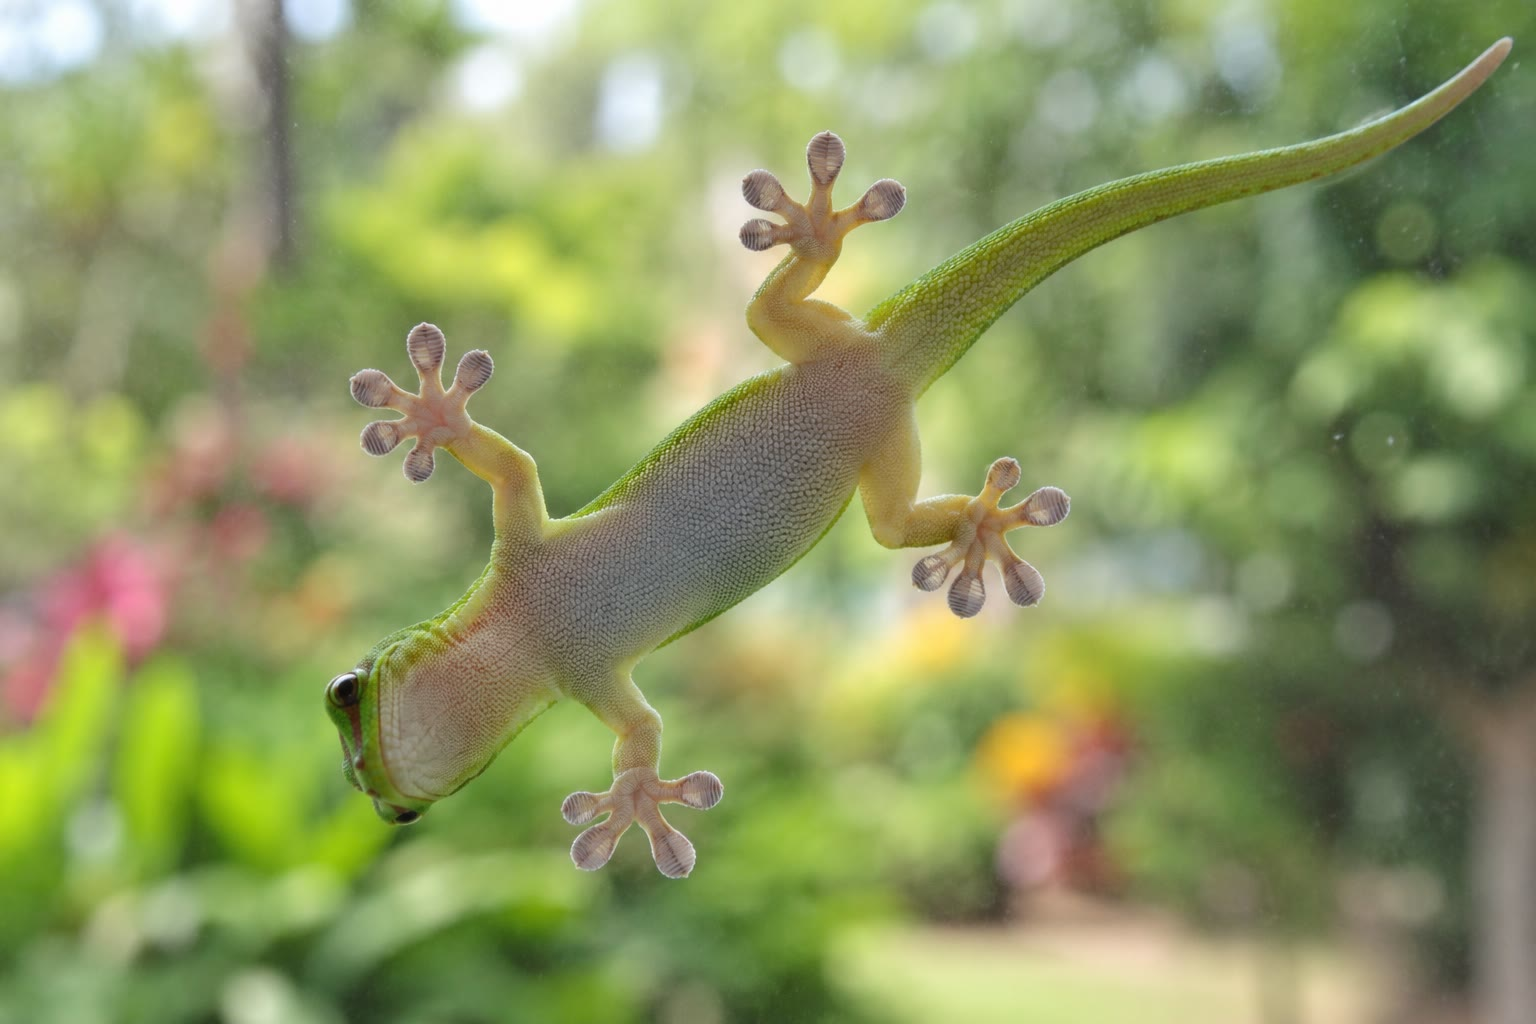
\includegraphics[width=0.5\linewidth]{images/book1/ai/g11-gecko-glass.jpg}

{\small وزغ على لوح زجاجي: وسائد أصابعه تتمسك بقوى بين
\omterm{def:g7:atoms-and-molecules:molecule}{الجزيئات}.}
\end{omfigure}

\section{الكهرسلبية}

\begin{definition}[الكهرسلبية]\label{def:g11:polarity-and-cohesion:electronegativity}
\emph{الكهرسلبية}\index{كهرسلبية} لعنصر تقيس شدة جذب ذراته، في \omterm{def:g7:atoms-and-molecules:molecule}{الجزيء}،
\omterm{def:g9:inside-the-atom:nucleus}{لإلكترونات} الروابط التي تتشارك فيها. وهي عدد بلا وحدة؛ ويمتد في السلّم المعتاد
من نحو 0.8 إلى نحو 4.
\end{definition}

\begin{omfigure}
% ledger: en:H, en:Li, en:Be, en:B, en:C, en:N, en:O, en:F, en:Na, en:Mg, en:Al, en:Si, en:P, en:S, en:Cl, en:K, en:Ca
\omperiodictable[upto=20, f block=false, cell=0.9cm, values={H/2.20,
  Li/0.98, Be/1.57, B/2.04, C/2.55, N/3.04, O/3.44, F/3.98, Na/0.93,
  Mg/1.31, Al/1.61, Si/1.90, P/2.19, S/2.58, Cl/3.16, K/0.82, Ca/1.00},
  highlight={F,O,N,Cl}]

{\small كهرسلبيات العناصر العشرين الأولى (سلّم باولنغ؛ ولا تُعطى قيمة للهيليوم
والنيون والأرغون، فهي لا تكوّن روابط هنا). والمظلَّلة: العناصر الأربعة الأشد
\omterm{def:g11:polarity-and-cohesion:electronegativity}{كهرسلبية}.}
\end{omfigure}

\begin{proposition}[الاتجاهات في الجدول]\label{prop:g11:polarity-and-cohesion:trends}
% ledger: en:F, en:Li, en:Cl, en:K
تزداد \omterm{def:g11:polarity-and-cohesion:electronegativity}{الكهرسلبية} من اليسار إلى اليمين على امتداد \omterm{def:g9:periodic-table-first-look:period}{الدورة} وتتناقص من الأعلى إلى
الأسفل في \omterm{def:g9:periodic-table-first-look:period}{الزمرة}. فالفلور (3.98) أشد العناصر \omterm{def:g11:polarity-and-cohesion:electronegativity}{كهرسلبية}؛ \omterm{def:g10:electron-shells:family}{والفلزات القلوية} أقلها
(الليثيوم 0.98، والبوتاسيوم 0.82).
\end{proposition}

\begin{proof}
نقرأ ذلك على الجدول: على امتداد \omterm{def:g9:periodic-table-first-look:period}{الدورة} 2، $0.98 < 1.57 < 2.04 < 2.55 < 3.04 <
3.44 < 3.98$؛ ونزولًا في \omterm{def:g9:periodic-table-first-look:period}{الزمرة} 17، الفلور $3.98$ فوق الكلور
$3.16$؛ ونزولًا في \omterm{def:g9:periodic-table-first-look:period}{الزمرة} 1، $2.20$ و$0.98$ و$0.93$ و$0.82$. (أما لماذا يكون الأمر
كذلك فيُشرح في كتاب السنة الجامعية الأولى.)
\end{proof}

\begin{history}[سلّم باولنغ، 1932]
بنى الكيميائي لينوس باولنغ أول سلّم \omterm{def:g11:polarity-and-cohesion:electronegativity}{للكهرسلبية} سنة 1932، انطلاقًا من طاقات
الروابط بين \omterm{def:g7:atoms-and-molecules:atom}{ذرات} مختلفة. وأعطى الفلور أكبر قيمة، ولا يزال السلّم المستعمل في
هذا الفصل يُسمّى باسمه.
\end{history}

\section{الروابط القطبية والجزيئات القطبية}

\begin{definition}[الرابطة القطبية، والشحنة الجزئية]\label{def:g11:polarity-and-cohesion:polar-bond}
\omterm{def:g10:lewis-and-shape:covalent-bond}{الرابطة التساهمية} بين ذرتين مختلفتي \omterm{def:g11:polarity-and-cohesion:electronegativity}{الكهرسلبية} \emph{رابطة قطبية}\index{رابطة قطبية}:
يكون الزوج المشترك أقرب إلى \omterm{def:g7:atoms-and-molecules:atom}{الذرة} الأشد \omterm{def:g11:polarity-and-cohesion:electronegativity}{كهرسلبية}. فتحمل تلك \omterm{def:g7:atoms-and-molecules:atom}{الذرة}
\emph{شحنة جزئية}\index{شحنة جزئية} سالبة صغيرة، يُرمز إليها بالرمز $\delta^-$،
وتحمل \omterm{def:g7:atoms-and-molecules:atom}{الذرة} الأخرى شحنة جزئية موجبة مساوية، $\delta^+$.
\end{definition}

\begin{proposition}[متى تكون الرابطة قطبية؟]\label{prop:g11:polarity-and-cohesion:polar-bond}
% ledger: en:C, en:H, en:O, en:Na, en:Cl
الرابطة بين ذرتين متماثلتين ليست قطبية. وبين ذرتين مختلفتين، كلما كبر فرق
\omterm{def:g11:polarity-and-cohesion:electronegativity}{الكهرسلبية} كانت الرابطة أشد قطبية؛ وكقاعدة تقريبية، يُعدّ الفرق الأصغر من نحو
0.4 (مثل \ce{C-H}، $2.55 - 2.20 = 0.35$) غير قطبي. وحين يكون الفرق كبيرًا جدًا
(مثل Na وCl، $3.16 - 0.93 = 2.23$) لا تتشارك الذرتان \omterm{def:g9:inside-the-atom:nucleus}{الإلكترونات} بل تنتقل:
فيكون المركب أيونيًا.
\end{proposition}

\begin{proof}
نقبله: فهو ينتج عن تعريف \omterm{def:g11:polarity-and-cohesion:electronegativity}{الكهرسلبية}، والعتبات
اصطلاحات.
\end{proof}

\begin{definition}[الجزيئات القطبية وغير القطبية]\label{def:g11:polarity-and-cohesion:polar-molecule}
يكون \omterm{def:g7:atoms-and-molecules:molecule}{الجزيء} \emph{جزيئًا قطبيًا}\index{جزيء قطبي} إذا لم ينطبق مركز شحناته
الجزئية الموجبة على مركز شحناته الجزئية السالبة؛ وإذا انطبقا كان
\emph{جزيئًا غير قطبي}\index{جزيء غير قطبي}.
\end{definition}

\begin{method}[هل الجزيء قطبي؟]\label{met:g11:polarity-and-cohesion:polar}
\begin{enumerate}
  \item ارسم \omterm{def:g10:lewis-and-shape:lewis-structure}{بنية لويس} وجد شكل \omterm{def:g7:atoms-and-molecules:molecule}{الجزيء}.
  \item علّم الروابط القطبية بالرمزين $\delta^+$ و$\delta^-$.
  \item إذا لم توجد \omterm{def:g11:polarity-and-cohesion:polar-bond}{رابطة قطبية} \omterm{def:g11:polarity-and-cohesion:polar-molecule}{فالجزيء غير قطبي}. وإلا فانظر إلى
        الشكل: إذا كانت الروابط القطبية مرتبة تناظريًا حول المركز تلاشت
        آثارها وكان \omterm{def:g11:polarity-and-cohesion:polar-molecule}{الجزيء غير قطبي}؛ وإلا كان
        قطبيًا.
\end{enumerate}
\end{method}

\begin{omfigure}
\begin{tikzpicture}[font=\small]
  % water
  \begin{scope}
    \node[aO] (o) at (0,0) {};
    \node[aH] (h1) at (-0.82,-0.6) {};
    \node[aH] (h2) at (0.82,-0.6) {};
    \begin{scope}[on background layer]
      \draw[bond] (o.center) -- (h1.center); \draw[bond] (o.center) -- (h2.center);
    \end{scope}
    \node[omThm] at (0,0.55) {$2\delta^-$};
    \node[omDef] at (-1.22,-0.5) {$\delta^+$};
    \node[omDef] at (1.22,-0.5) {$\delta^+$};
    \fill[omDef] (0,-0.6) circle (0.06);
    \fill[omThm] (0,0) circle (0.06);
    \draw[densely dotted, black!60] (-0.82,-0.6) -- (0.82,-0.6);
    \draw[<-, black!60] (0.08,-0.64) -- (1.55,-1.05) node[right, align=left,
      font=\footnotesize] {مركز\\ \foreignlanguage{arabic}{الشحنات $\delta^+$}};
    \node[align=center, anchor=north] at (0,-1.8) {الماء: منحنٍ، \textbf{قطبي}};
  \end{scope}
  % carbon dioxide
  \begin{scope}[xshift=6cm]
    \node[aO] (o1) at (-1.15,0) {};
    \node[aC] (c) at (0,0) {};
    \node[aO] (o2) at (1.15,0) {};
    \begin{scope}[on background layer]
      \draw[bond, double, double distance=1.6pt] (o1.center) -- (c.center);
      \draw[bond, double, double distance=1.6pt] (c.center) -- (o2.center);
    \end{scope}
    \node[omThm] at (-1.15,0.55) {$\delta^-$};
    \node[omThm] at (1.15,0.55) {$\delta^-$};
    \node[omDef] at (0,0.55) {$2\delta^+$};
    \draw[->, omProp, thick] (-0.25,-0.45) -- (-1.0,-0.45);
    \draw[->, omProp, thick] (0.25,-0.45) -- (1.0,-0.45);
    \node[align=center, anchor=north] at (0,-1.8) {ثنائي أكسيد الكربون: خطي،\\
      \textbf{غير قطبي}};
  \end{scope}
\end{tikzpicture}

{\small في الماء يجعل الشكل المنحني مركز الشحنات الجزئية الموجبة (بين ذرتي
الهيدروجين) تحت \omterm{def:g7:atoms-and-molecules:atom}{ذرة} الأكسجين: \omterm{def:g11:polarity-and-cohesion:polar-molecule}{فالجزيء قطبي}. وفي ثنائي أكسيد الكربون تشد الرابطتان
القطبيتان في اتجاهين متعاكسين (السهمان) فتتلاشيان: وينطبق مركزا الشحنات على
\omterm{def:g7:atoms-and-molecules:atom}{ذرة} الكربون.}
\end{omfigure}


\begin{example}[أربعة جزيئات]\label{ex:g11:polarity-and-cohesion:four}
لكلوريد الهيدروجين \ce{HCl} \omterm{def:g11:polarity-and-cohesion:polar-bond}{رابطة قطبية} واحدة، فهو قطبي، والكلور
$\delta^-$. والأمونياك \ce{NH3}، وهو هرم من ثلاث روابط \ce{N-H} قطبية،
قطبي، والنيتروجين $\delta^-$. وليس للميثان \ce{CH4} إلا روابط \ce{C-H} شبه
غير قطبية: فهو غير قطبي. ولرباعي كلورو الميثان \ce{CCl4} أربع روابط
\ce{C-Cl} قطبية، لكنها على رؤوس رباعي أوجه منتظم: فتتلاشى آثارها ويكون \omterm{def:g11:polarity-and-cohesion:polar-molecule}{الجزيء
غير قطبي}.
\end{example}

\section{تآثرات فان دير فالس}

\begin{definition}[تآثر فان دير فالس]\label{def:g11:polarity-and-cohesion:van-der-waals}
\emph{تآثر فان دير فالس}\index{تآثر فان دير فالس} تجاذب ضعيف بين \omterm{def:g7:atoms-and-molecules:molecule}{جزيئات}
متجاورة، موجود بين كل \omterm{def:g7:atoms-and-molecules:molecule}{الجزيئات}، قطبية كانت أم لا: \omterm{def:g9:inside-the-atom:nucleus}{فإلكترونات} كل \omterm{def:g7:atoms-and-molecules:molecule}{جزيء} تتحرك
باستمرار، والشحنات غير المتوازنة اللحظية في \omterm{def:g7:atoms-and-molecules:molecule}{جزيء} تجذب شحنات جيرانه. وبين
\omterm{def:g7:atoms-and-molecules:molecule}{الجزيئات} القطبية تضيف الشحنات الجزئية الدائمة تجاذبًا
آخر.
\end{definition}


\begin{proposition}[الجزيئات الأكبر تتجاذب أكثر]\label{prop:g11:polarity-and-cohesion:size}
تكبر تآثرات فان دير فالس مع حجم \omterm{def:g7:atoms-and-molecules:molecule}{الجزيئات}، أي مع عدد إلكتروناتها؛ وبين \omterm{def:g7:atoms-and-molecules:molecule}{جزيئات}
متشابهة تكون للأكبر منها درجات الانصهار والغليان
الأعلى.
\end{proposition}

\begin{proof}
نقبله: فالسحابة الإلكترونية الأكبر أسهل تشوّهًا، فتكون شحناتها اللحظية أكبر،
ويكون تلامسها مع جيرانها أكثر.
\end{proof}

\begin{example}[الهالوجينات]\label{ex:g11:polarity-and-cohesion:halogens}
% ledger: bp:F2, bp:Cl2, bp:Br2, bp:I2 (K values converted)
\omterm{def:g7:atoms-and-molecules:molecule}{الجزيئات} \ce{F2} و\ce{Cl2} و\ce{Br2} و\ce{I2} كلها غير قطبية وأكبر
فأكبر. وترتفع درجات غليانها معها:
\qty{-188}{\celsius} و\qty{-34}{\celsius} و\qty{59}{\celsius}
و\qty{184}{\celsius}. وفي درجة حرارة الغرفة يكون الفلور والكلور غازين، والبروم
سائلًا، واليود جسمًا صلبًا.
\end{example}

\begin{remark}[الوزغ]\label{rem:g11:polarity-and-cohesion:gecko}
\omterm{def:g11:polarity-and-cohesion:van-der-waals}{تآثر فان دير فالس} الواحد ضئيل، لكن التآثرات تتراكم. فوسائد أصابع الوزغ مغطاة
بسجادة كثيفة من شعيرات مجهرية، ينقسم كل منها إلى أطراف أدق، تقترب من الزجاج
بما يكفي لتعمل تآثرات فان دير فالس على مساحة كلية كبيرة جدًا.
\end{remark}

\section{الروابط الهيدروجينية}

\begin{definition}[الرابطة الهيدروجينية]\label{def:g11:polarity-and-cohesion:hydrogen-bond}
\emph{الرابطة الهيدروجينية}\index{رابطة هيدروجينية} تجاذب بين \omterm{def:g7:atoms-and-molecules:atom}{ذرة} هيدروجين
مرتبطة \omterm{def:g7:atoms-and-molecules:atom}{بذرة} شديدة \omterm{def:g11:polarity-and-cohesion:electronegativity}{الكهرسلبية} (نيتروجين، أو أكسجين، أو فلور)، تحمل $\delta^+$
واضحة، \omterm{def:g10:lewis-and-shape:lone-pair}{وزوج حر} \omterm{def:g7:atoms-and-molecules:atom}{لذرة} نيتروجين أو أكسجين أو فلور أخرى، كثيرًا ما تكون في \omterm{def:g7:atoms-and-molecules:molecule}{جزيء}
مجاور. وتُرسم بخط متقطع، \omterm{def:g7:atoms-and-molecules:atom}{والذرات} الثلاث المعنية تكاد تكون على خط
مستقيم.
\end{definition}

\begin{omfigure}
\begin{tikzpicture}[font=\small]
  % central water molecule and four neighbours, H-bonds dashed
  \newcommand{\water}[4]{% name, x, y, rotation
    \begin{scope}[shift={(#2,#3)}, rotate=#4]
      \node[aO] (#1o) at (0,0) {};
      \node[aH] (#1a) at (-0.6,-0.45) {};
      \node[aH] (#1b) at (0.6,-0.45) {};
    \end{scope}
    \begin{scope}[on background layer]
      \draw[bond] (#1o.center) -- (#1a.center); \draw[bond] (#1o.center) -- (#1b.center);
    \end{scope}}
  \water{m}{0}{0}{0}
  \water{p}{-1.62}{-1.215}{0}
  \water{q}{1.62}{-1.215}{0}
  \water{r}{-1.435}{1.435}{-8.13}
  \water{s}{1.435}{1.435}{8.13}
  % H-bonds: m's H to p's O and q's O; r's and s's H to m's O
  \draw[dashed, omDef, thick] (ma) -- (po);
  \draw[dashed, omDef, thick] (mb) -- (qo);
  \draw[dashed, omDef, thick] (rb) -- (mo);
  \draw[dashed, omDef, thick] (sa) -- (mo);
\end{tikzpicture}

{\small الروابط الهيدروجينية (المتقطعة) حول \omterm{def:g7:atoms-and-molecules:molecule}{جزيء} ماء في الماء السائل: ترتبط ذرتا
الهيدروجين فيه بذرتي أكسجين جزيئين مجاورين، ويستقبل الزوجان الحران \omterm{def:g7:atoms-and-molecules:atom}{لذرة}
أكسجينه ذرتي هيدروجين جزيئين آخرين.}
\end{omfigure}


\begin{example}[الإيثانول والبروبان]\label{ex:g11:polarity-and-cohesion:ethanol}
% ledger: bp:C2H5OH, bp:C3H8 (K values converted)
للإيثانول والبروبان \omterm{def:g7:atoms-and-molecules:molecule}{جزيئات} متقاربة جدًا في الحجم: فصيغة الأول \ce{CH3-CH2-OH}
وكتلته المولية \qty{46.0}{g/mol}، وصيغة الثاني \ce{CH3-CH2-CH3} وكتلته المولية \qty{44.0}{g/mol}. ومع ذلك يغلي
الإيثانول عند \qty{78}{\celsius} والبروبان عند
\qty{-42}{\celsius}. \omterm{def:g7:atoms-and-molecules:molecule}{فجزيئات} الإيثانول، بمجموعتها \ce{O-H}، تكوّن روابط
هيدروجينية بعضها مع بعض؛ أما \omterm{def:g7:atoms-and-molecules:molecule}{جزيئات} البروبان فلا تستطيع.
\end{example}

\section{تماسك الأجسام الصلبة والسوائل}

\begin{definition}[الجسم الصلب الجزيئي]\label{def:g11:polarity-and-cohesion:molecular-solid}
\emph{الجسم الصلب الجزيئي}\index{جسم صلب جزيئي} جسم صلب مكوّن من \omterm{def:g7:atoms-and-molecules:molecule}{جزيئات} يشد
بعضها بعضًا بتآثرات فان دير فالس، وبروابط هيدروجينية حيث أمكن. فالجليد واليود
الصلب والسكر أجسام صلبة جزيئية.
\end{definition}

\begin{proposition}[التماسك وتغير الحالة]\label{prop:g11:polarity-and-cohesion:cohesion}
كلما اشتد التجاذب بين جسيمات المادة ارتفعت درجتا انصهارها وغليانها. وبترتيب
تزايد الشدة: تآثرات فان دير فالس، ثم الروابط الهيدروجينية، ثم التجاذب بين
\omterm{def:g9:ions:ion}{أيونات} الجسم الصلب الأيوني.
\end{proposition}

\begin{proof}
نقبله: فالانصهار والغليان يباعدان الجسيمات رغم هذا التجاذب، وهذا يتطلب طاقة
أكبر، أي درجة حرارة أعلى، حين يكون التجاذب
أشد.
\end{proof}

\begin{example}[ثلاثة أجسام صلبة]\label{ex:g11:polarity-and-cohesion:three}
% ledger: mp:NaCl, mp:water
كلوريد الصوديوم، وهو جسم صلب أيوني، ينصهر عند \qty{801}{\celsius}؛ والجليد،
الذي تمسكه الروابط الهيدروجينية، عند \qty{0}{\celsius}؛ والميثان الصلب، الذي
لا تمسكه إلا تآثرات فان دير فالس بين \omterm{def:g7:atoms-and-molecules:molecule}{جزيئات} صغيرة، عند درجة أدنى بكثير من
\qty{-150}{\celsius}.
\end{example}

\begin{omfigure}
\begin{tikzpicture}
\begin{axis}[width=0.6\linewidth, height=7cm, xmin=1.7, xmax=5.3,
    ymin=-190, ymax=120, xtick={2,3,4,5}, xlabel={الدورة},
    ylabel={\foreignlanguage{arabic}{درجة الغليان \babelsublr{(\si{\celsius})}}}, axis lines*=left,
    ymajorgrids, grid style={gray!20}, tick label style={font=\small},
    label style={font=\small},
    legend style={font=\small, at={(1.02,0.5)}, anchor=west, draw=none},
    legend cell align=left]
  % ledger: bp:CH4, bp:SiH4, bp:GeH4, bp:NH3, bp:PH3, bp:AsH3, bp:SbH3, bp:H2O, bp:H2S, bp:H2Se, bp:HF, bp:HCl, bp:HBr, bp:HI (K values converted to degC)
  \addplot[thick, mark=*, black!70] coordinates {(2,-162.2) (3,-112) (4,-88.1)};
  \addplot[thick, mark=square*, omMeth] coordinates {(2,-33.4) (3,-87.8) (4,-62.5) (5,-18.4)};
  \addplot[thick, mark=triangle*, mark size=3pt, omThm] coordinates {(2,100.0) (3,-60.3) (4,-41.3)};
  \addplot[thick, mark=diamond*, mark size=3pt, omDef] coordinates {(2,19.6) (3,-85.1) (4,-66.4) (5,-35.1)};
  \legend{{\foreignlanguage{arabic}{الزمرة \babelsublr{14} \babelsublr{(\ce{CH4} \dots)}}}, {\foreignlanguage{arabic}{الزمرة \babelsublr{15} \babelsublr{(\ce{NH3} \dots)}}},
    {\foreignlanguage{arabic}{الزمرة \babelsublr{16} \babelsublr{(\ce{H2O} \dots)}}}, {\foreignlanguage{arabic}{الزمرة \babelsublr{17} \babelsublr{(\ce{HF} \dots)}}}}
  \node[font=\footnotesize, anchor=west] at (axis cs:2.05,100) {\ce{H2O}};
  \node[font=\footnotesize, anchor=west] at (axis cs:2.05,19.6) {\ce{HF}};
  \node[font=\footnotesize, anchor=west] at (axis cs:2.05,-33.4) {\ce{NH3}};
  \node[font=\footnotesize, anchor=north west] at (axis cs:2.05,-166) {\ce{CH4}};
\end{axis}
\end{tikzpicture}

{\small درجات غليان مركبات الهيدروجين مع عناصر الزمر من 14 إلى 17. ترتفع في كل
\omterm{def:g9:periodic-table-first-look:period}{زمرة} مع حجم \omterm{def:g7:atoms-and-molecules:molecule}{الجزيء}، ما عدا العضو الأول في الزمر 15 و16 و17، فقيمه أعلى بكثير
من المتوقع: فالأمونياك والماء وفلوريد الهيدروجين تكوّن روابط هيدروجينية. (ولا
تُمثَّل قيمة حيث لا تعطي المصادر المستعملة
قيمة.)}
\end{omfigure}

\begin{remark}[الجليد والثلج]\label{rem:g11:polarity-and-cohesion:ice}
في الجليد يرتبط كل \omterm{def:g7:atoms-and-molecules:molecule}{جزيء} ماء بروابط هيدروجينية بأربعة جيران، في شبكة مفتوحة من
حلقات سداسية. وهذه الشبكة تترك فراغًا أكبر مما في الماء السائل، حيث تتكسر الروابط
وتتكوّن باستمرار: فالجليد أقل كثافة من الماء ويطفو. والتناظر السداسي لبلورات
الثلج يعكس الحلقات السداسية للشبكة.
\end{remark}

\begin{omfigure}
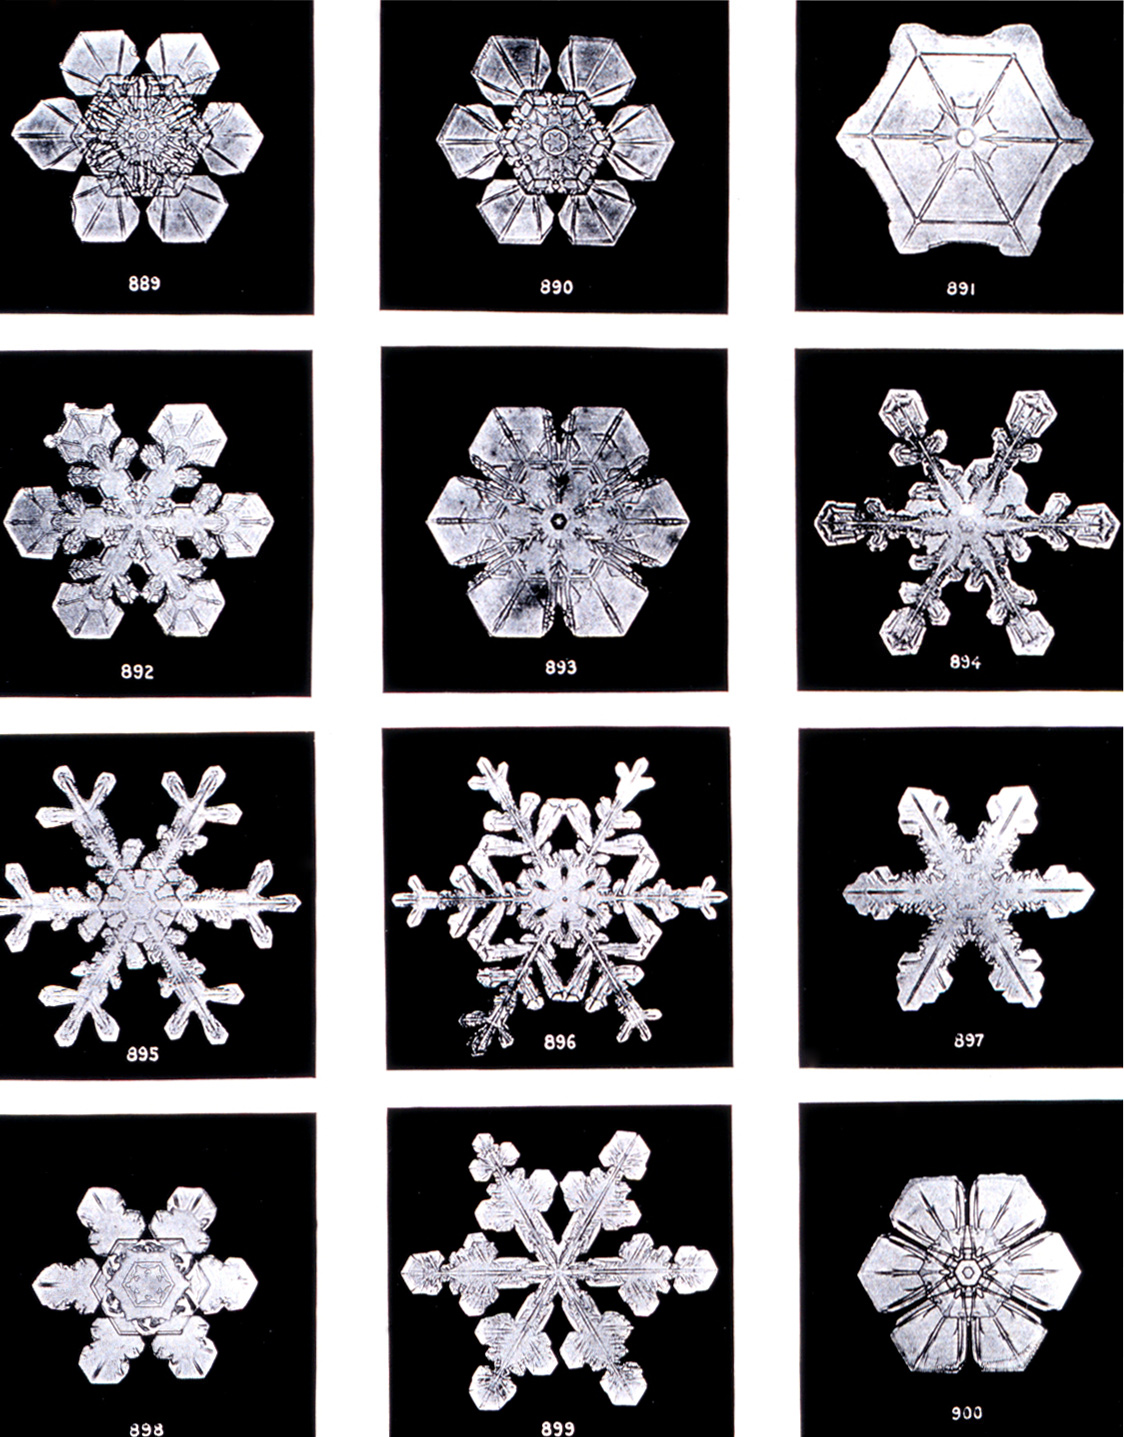
\includegraphics[width=0.36\linewidth]{images/book1/snowflakes.jpg}

{\small بلورات ثلج صوّرها ويلسون بنتلي في أوائل القرن العشرين: لكل منها ستة
فروع.}
\end{omfigure}

\section{تمارين}


\begin{exercise}[$\star$]\label{exo:g11:polarity-and-cohesion:1}
في الروابط \ce{H-Cl} و\ce{O-H} و\ce{C-O}، أي \omterm{def:g7:atoms-and-molecules:atom}{ذرة} تحمل \omterm{def:g11:polarity-and-cohesion:polar-bond}{الشحنة الجزئية}
$\delta^-$؟ استعمل جدول الكهرسلبيات.
\end{exercise}

\begin{exercise}[$\star$]\label{exo:g11:polarity-and-cohesion:2}
أي هذه الروابط قطبية: \ce{H-H} و\ce{C-H} و\ce{O-H} و\ce{N-H}
و\ce{Cl-Cl} و\ce{C-Cl}؟ أعطِ فرق \omterm{def:g11:polarity-and-cohesion:electronegativity}{الكهرسلبية} لكل
منها.
\end{exercise}

\begin{exercise}[$\star$]\label{exo:g11:polarity-and-cohesion:3}
أي العنصرين أشد \omterm{def:g11:polarity-and-cohesion:electronegativity}{كهرسلبية} في كل زوج: النيتروجين أم الفوسفور؛ والأكسجين أم
الكبريت؛ والكربون أم النيتروجين؛ والصوديوم أم المغنيسيوم؟ وأي اتجاه في الجدول
يوضحه كل زوج؟
\end{exercise}

\begin{exercise}[$\star$]\label{exo:g11:polarity-and-cohesion:4}
أي \omterm{def:g7:atoms-and-molecules:molecule}{الجزيئات} \ce{CH4} و\ce{NH3} و\ce{H2O} و\ce{HCl} يستطيع أن يكوّن روابط
هيدروجينية بين جزيئاته؟ علّل.
\end{exercise}

\begin{exercise}[$\star$]\label{exo:g11:polarity-and-cohesion:5}
هل توجد تجاذبات بين \omterm{def:g7:atoms-and-molecules:molecule}{جزيئات} الميثان غير القطبية؟ ولماذا يبقى الميثان مع ذلك غازًا
في درجة حرارة الغرفة؟
\end{exercise}

\begin{exercise}[$\star\star$]\label{exo:g11:polarity-and-cohesion:6}
قل عن كل \omterm{def:g7:atoms-and-molecules:molecule}{جزيء} هل هو قطبي: ثنائي كلورو الميثان \ce{CH2Cl2}
(رباعي الأوجه)، ورباعي كلورو الميثان \ce{CCl4}، والأمونياك \ce{NH3}، وثنائي
أكسيد الكربون \ce{CO2}، وثلاثي فلوريد البور \ce{BF3} (مثلث مستوٍ والبور في
مركزه).
\end{exercise}

\begin{exercise}[$\star\star$]\label{exo:g11:polarity-and-cohesion:7}
في الميثانول، \ce{CH3-OH}، أي \omterm{def:g7:atoms-and-molecules:atom}{ذرة} هيدروجين يمكن أن تُعطى في \omterm{def:g11:polarity-and-cohesion:hydrogen-bond}{رابطة
هيدروجينية}؟ وأي \omterm{def:g7:atoms-and-molecules:atom}{ذرة} يمكن أن تستقبلها؟ وهل تستطيع \omterm{def:g7:atoms-and-molecules:molecule}{جزيئات} الميثانول والماء أن تكوّن
روابط هيدروجينية بعضها مع بعض؟ ارسم واحدة.
\end{exercise}

\begin{exercise}[$\star\star$]\label{exo:g11:polarity-and-cohesion:8}
اشرح لماذا ترتفع درجات الغليان بالترتيب \ce{CH4} <
\ce{SiH4} < \ce{GeH4}.
\end{exercise}

\begin{exercise}[$\star\star$]\label{exo:g11:polarity-and-cohesion:9}
في مخطط درجات غليان الهيدريدات، أي \omterm{def:g9:periodic-table-first-look:period}{زمرة} لا تُظهر قيمة غير عادية لعضوها
الأول؟ ولماذا؟
\end{exercise}

\begin{exercise}[$\star\star$]\label{exo:g11:polarity-and-cohesion:10}
% ledger: en:H, en:Cl, en:Br, en:I, bp:HCl, bp:HBr, bp:HI
الروابط \ce{H-Cl} و\ce{H-Br} و\ce{H-I} أقل فأقل قطبية (كهرسلبيات الكلور والبروم
واليود 3.16 و2.96 و2.66)، ومع ذلك ترتفع درجات الغليان: \qty{-85}{\celsius}
و\qty{-66}{\celsius} و\qty{-35}{\celsius}. أي التآثرين يغلب،
ولماذا؟
\end{exercise}

\begin{exercise}[$\star\star$]\label{exo:g11:polarity-and-cohesion:11}
في درجة حرارة الغرفة يكون الكلور غازًا واليود جسمًا صلبًا، مع أن كليهما مكوّن من
\omterm{def:g7:atoms-and-molecules:molecule}{جزيئات} غير قطبية \ce{X2}. علّل.
\end{exercise}

\begin{exercise}[$\star\star\star$]\label{exo:g11:polarity-and-cohesion:12}
% ledger: bp:C2H5OH, bp:CH3OCH3, bp:C3H8
للإيثانول \ce{CH3-CH2-OH}، والميثوكسي ميثان \ce{CH3-O-CH3}، والبروبان
\ce{CH3-CH2-CH3} \omterm{def:g10:the-mole:molar-mass}{الكتلة المولية} نفسها تقريبًا. وهي تغلي عند
\qty{78}{\celsius} و\qty{-25}{\celsius} و\qty{-42}{\celsius}. أيها
قطبي؟ وأيها يكوّن روابط هيدروجينية بين جزيئاته؟ اشرح
الترتيب.
\end{exercise}

\begin{exercise}[$\star\star\star$]\label{exo:g11:polarity-and-cohesion:13}
في الجليد يرتبط كل \omterm{def:g7:atoms-and-molecules:molecule}{جزيء} ماء بروابط هيدروجينية بأربعة جيران، في شبكة مفتوحة؛
وفي الماء السائل تتكسر الشبكة باستمرار وتنهار جزئيًا. اشرح لماذا يطفو الجليد على
الماء. ولماذا يهم ذلك أسماك بحيرة
متجمدة؟
\end{exercise}

\begin{exercise}[$\star\star\star$]\label{exo:g11:polarity-and-cohesion:14}
رتّب بحسب تزايد درجة الانصهار، وعلّل بالتجاذب بين الجسيمات: كلوريد البوتاسيوم
\ce{KCl}، والجليد \ce{H2O}، والميثان الصلب
\ce{CH4}.
\end{exercise}

\begin{exercise}[$\star\star\star$]\label{exo:g11:polarity-and-cohesion:15}
% ledger: en:F, en:O, bp:HF, bp:H2O
الفلور أشد \omterm{def:g11:polarity-and-cohesion:electronegativity}{كهرسلبية} من الأكسجين، فالرابطة \ce{H-F} أشد قطبية من الرابطة
\ce{O-H}. ومع ذلك يغلي الماء عند \qty{100}{\celsius} وفلوريد الهيدروجين عند
\qty{20}{\celsius}. عُدّ \omterm{def:g7:atoms-and-molecules:atom}{ذرات} الهيدروجين التي يستطيع كل \omterm{def:g7:atoms-and-molecules:molecule}{جزيء} أن يعطيها والأزواج
الحرة التي يستطيع أن يستقبل بها، واشرح.
\end{exercise}

\section{مسألة: لماذا يغلي الماء عند \texorpdfstring{\qty{100}{\celsius}}{100 درجة مئوية}؟}

\begin{problem}[{مسألة نهاية الأسبوع --- لولا الروابط الهيدروجينية، عند أي درجة
حرارة كان الماء سيغلي؟}]
\label{pb:g11:polarity-and-cohesion:1}
% ledger: en:H, en:O, en:S, en:Se, bp:H2O, bp:H2S, bp:H2Se, bp:CH4, bp:SiH4, bp:GeH4, bp:HCl, bp:HBr, bp:HF, bp:NH3, bp:PH3, bp:AsH3
الأكسجين والكبريت والسيلينيوم في \omterm{def:g9:periodic-table-first-look:period}{الزمرة} نفسها من الجدول، والثلاثة تكوّن مركبًا مع
الهيدروجين: \ce{H2O} و\ce{H2S} و\ce{H2Se}. وفي كل \omterm{def:g9:periodic-table-first-look:period}{زمرة} من الهيدريدات ترتفع
درجات الغليان عادة مع حجم \omterm{def:g7:atoms-and-molecules:molecule}{الجزيء}. والماء يخالف القاعدة. فبكم؟

\medskip
\noindent\textbf{الجزء الأول --- ثلاثة \omterm{def:g7:atoms-and-molecules:molecule}{جزيئات}.}
\begin{enumerate}
  \item ارسم بنى لويس \omterm{def:g7:atoms-and-molecules:molecule}{للجزيئات} \ce{H2O} و\ce{H2S} و\ce{H2Se}.
        لماذا هي متشابهة؟
  \item احسب كتلها المولية.
  \item احسب فروق \omterm{def:g11:polarity-and-cohesion:electronegativity}{الكهرسلبية} للروابط
        \ce{O-H} و\ce{S-H} و\ce{Se-H} (الأكسجين 3.44، والكبريت 2.58،
        والسيلينيوم 2.55، والهيدروجين 2.20). أي الروابط قطبية بوضوح؟
  \item ما شكل \omterm{def:g7:atoms-and-molecules:molecule}{الجزيئات} الثلاثة؟ وهل هي قطبية؟
  \item عُدّ \omterm{def:g9:inside-the-atom:nucleus}{إلكترونات} كل \omterm{def:g7:atoms-and-molecules:molecule}{جزيء}. أيها له أقوى تآثرات فان
        دير فالس؟
\end{enumerate}

\medskip
\noindent\textbf{الجزء الثاني --- الروابط الهيدروجينية.}
\begin{enumerate}[resume]
  \item أي المركبات الثلاثة يكوّن روابط هيدروجينية بين
        جزيئاته؟ ولماذا لا يكوّنها الآخران؟
  \item كم \omterm{def:g11:polarity-and-cohesion:hydrogen-bond}{رابطة هيدروجينية} يستطيع \omterm{def:g7:atoms-and-molecules:molecule}{جزيء} ماء واحد أن يشارك فيها على
        الأكثر؟ ارسمها.
  \item أي التآثرات تمسك \omterm{def:g7:atoms-and-molecules:molecule}{جزيئات} كبريتيد الهيدروجين بعضها ببعض
        في السائل؟
\end{enumerate}

\medskip
\noindent\textbf{الجزء الثالث --- الاتجاه.}
\begin{enumerate}[resume]
  \item يغلي كبريتيد الهيدروجين عند \qty{212.9}{K} وسيلينيد الهيدروجين عند
        \qty{-41.3}{\celsius}. عبّر عن الأولى بالدرجات المئوية
        ($\theta = T - 273.15$).
  \item بكم ترتفع درجة الغليان من \omterm{def:g9:periodic-table-first-look:period}{الدورة} 3
        (\ce{H2S}) إلى \omterm{def:g9:periodic-table-first-look:period}{الدورة} 4 (\ce{H2Se})؟
  \item لماذا ترتفع؟
  \item بافتراض الارتفاع نفسه من \omterm{def:g9:periodic-table-first-look:period}{الدورة} 2 إلى \omterm{def:g9:periodic-table-first-look:period}{الدورة} 3، عند أي درجة
        حرارة كان سيغلي \ce{H2O} «عادي»؟
  \item اختبر الطريقة على \omterm{def:g9:periodic-table-first-look:period}{الزمرة} 14: يغلي \ce{SiH4} عند
        \qty{-112}{\celsius} و\ce{GeH4} عند \qty{-88.1}{\celsius}.
        تنبأ بدرجة غليان \ce{CH4} وقارنها بالدرجة
        الحقيقية، \qty{-162}{\celsius}. هل الاستقراء دقيق؟
  \item افعل الشيء نفسه \omterm{def:g9:periodic-table-first-look:period}{للزمرة} 17 (\ce{HCl} \qty{-85.1}{\celsius}،
        و\ce{HBr} \qty{-66.4}{\celsius}) وقارن بالمركب \ce{HF}،
        \qty{19.6}{\celsius}.
\end{enumerate}

\medskip
\noindent\textbf{الجزء الرابع --- الفجوة.}
\begin{enumerate}[resume]
  \item يغلي الماء حقًا عند \qty{100}{\celsius}. ما حجم الفجوة
        بين القيمة الحقيقية والقيمة المستقرأة؟
  \item السؤال نفسه للأمونياك، باستعمال \ce{PH3} \qty{-87.8}{\celsius}
        و\ce{AsH3} \qty{-62.5}{\celsius}؛ والأمونياك يغلي حقًا عند
        \qty{-33.4}{\celsius}.
  \item رتّب الماء وفلوريد الهيدروجين والأمونياك بحسب حجم
        فجوتها، وفسّر الترتيب بعدّ الروابط الهيدروجينية.
  \item لولا الروابط الهيدروجينية، هل كان الماء جسمًا صلبًا أم سائلًا أم غازًا
        في درجة حرارة الغرفة؟ وماذا كان سيعني ذلك للأرض؟
  \item لماذا لا يعدو جواب السؤال 12 أن يكون تقديرًا؟
  \item اذكر الجواب النهائي: عند أي درجة حرارة تقريبًا كان الماء سيغلي لولا
        الروابط الهيدروجينية؟
\end{enumerate}
\end{problem}
